\chapter{Métodos de \textit{Kernel} para Regressão} \label{chapter:kernel-methods}

Um dos principais desafios -- e objetivos -- do aprendizado de máquinas é encontrar informações inerentes de um problema, de forma que seu uso torne-se fator chave durante o processo de aprendizagem. Modelos lineares buscam tais informações através de correlações entre as características escolhidas para descrever o objeto de estudo. A teoria e gama de aplicações de modelos lineares têm sido bastante estudadas e analisadas por décadas, e hoje constituem um arcabouço bem definido no campo de AM. Entretanto, a grande ocorrência de fenômenos não-lineares em problemas do mundo real traz a necessidade de criação de modelos mais complexos.

Ao decorrer das últimas décadas, o uso de métodos de \textit{kernel} tem se mostrado bem sucedido ao permitir a criação de extensões não-lineares de clássicos modelos lineares \cite{abrahamsen2013}. A ideia básica por trás de métodos de \textit{kernel} é realizar um mapeamento do problema original para um espaço de alta -- ou até infinita -- dimensão, chamado de espaço de características, onde métodos lineares são utilizados para buscar as relações entre os padrões. Embora seu uso tenha se popularizado em anos recentes, o trabalho inicial na área costuma ser creditado a \citeonline{aizerman1964}, que utilizando o teorema de Mercer e RKHS, criaram algo muito próximo do que hoje é chamado de truque do \textit{kernel} \cite{schlkopf2004}.

O truque do \textit{kernel} permite a criação de eficientes métodos aplicáveis tanto para problemas de aprendizagem supervisionada quanto não-supervisionada. De particular interesse desta monografia, são as aplicações em problemas de regressão. Entre os métodos estado-da-arte, os membros mais conhecidos são: (\textit{i}) \textit{support vector regression} (SVR) \cite{smola1997}, cuja formulação é derivada da teoria do aprendizado estatístico \cite{vapnik1995,vapnik1998}; (\textit{ii}) \textit{least squares support vector regression} (LSSVR) \cite{suykens2002}, uma formulação simplificada do SVR; (\textit{iii}) \textit{kernel ridge regression} (KRR) \cite{saunders1998}, que possui uma formulação semelhante à das LSSVR; e por fim, (\textit{iv}) \textit{gaussian processes} (GP) \cite{rasmussen2006}, cuja formulação advém da teoria dos processos estocásticos.

Este capítulo descreve como a teoria de métodos de \textit{kernel} é utilizada no contexto da \textit{\textit{ridge regression}} para a criação do método KRR. Para isso, a seção \ref{sec:linreg} discute modelos de regressão linear, bem como apresenta como o método dos mínimos quadrados é utilizado para estimar %-- de maneira não-enviesada --
os coeficientes de regressão. A seção \ref{sec:ridge} apresenta a \textit{ridge regression} como um método de penalização da soma dos erros quadráticos. Na seção \ref{sec:kernel-trick} é mostrado como o truque do \textit{kernel} é utilizado para a formulação do KRR. Por fim, a seção \ref{sec:gkr} apresenta a proposta deste trabalho, denominada \textit{Genetic Kernels for Regression} (GKR).

\section{Regressão linear} \label{sec:linreg}
% Análise de regressão é uma técnica de estatística para investigação e modelagem de relacionamentos entre variáveis \cite{montgomery2012}. Através dessas variáveis podemos representar o comportamento de um objeto de interesse. Um dos modelos mais simples e utilizados para análise de regressão é descrito pela equação
Modelos de regressão são procedimentos estatísticos que permitem estimar relações entre variáveis, onde através destas podemos representar o comportamento de um objeto de interesse. Um dos modelos mais utilizados em problemas de regressão é descrito como

\begin{equation}
    \label{ch2:eq1}
    y = f(\mathbf{x}) = \mathbf{w}^{\top}\mathbf{x} = \sum_{j=1}^{p}{w_j \cdot x_j}
\end{equation}

Usualmente, variáveis à esquerda ($y$) da equação de regressão são chamadas de variáveis dependentes, enquanto as do lado direito ($\mathbf{x}$) são chamadas de variáveis independentes. Entretanto, \citeonline{montgomery2012} argumentam que tais nomenclaturas podem gerar confusão com o conceito de independência estatística. Dessa forma, nomearemos as variáveis da seguinte forma:

\begin{itemize}
    \item variáveis dependentes $\rightarrow$ variáveis de regressão;% (ou predição);
    \item variáveis independentes $\rightarrow$ variáveis de resposta.
\end{itemize}

De modo geral, o objetivo de um modelo de regressão é encontrar uma função que melhor interpole um conjunto de treinamento $\mathcal{D} = \{(\mathbf{x}_i, y_i)\}^{n}_{i=1}$ composto de pontos $\mathbf{x}_i$ extraídos de $\mathcal{X} \subseteq \mathbb{R}^p$ e $y_i$ extraídos de $\mathcal{Y} \subseteq \mathbb{R}$. Vale salientar que tanto neste capítulo, quanto no restante desta monografia, denotamos $\mathbf{x} = [x_1,x_2,\ldots,x_p]$ como o vetor de entrada p-dimensional e $\mathbf{w}^{\top}$ como o vetor transposto de $\mathbf{w} \in \mathbb{R}^p$. Quando a equação (\ref{ch2:eq1}) possui apenas uma variável de regressão, o modelo é chamado de \textbf{regressão linear simples}; quando possui duas ou mais variáveis, é chamado de \textbf{regressão linear múltipla}.

Em termos geométricos, um modelo de regressão linear posiciona um hiperplano de modo que este ajuste-se da melhor forma possível aos $n$ padrões de treinamento. A Figura \ref{fig:ch2-linreg} apresenta dois exemplos: \ref{fig:ch2-linreg1} caso unidimensional, $p = 1$, onde o hiperplano toma forma de uma linha reta; e \ref{fig:ch2-linreg2} caso bidimensional, $p = 2$, onde o hiperplano toma forma de um plano no $\mathbb{R}^2$.

\begin{figure}[ht]
    \caption{Hiperplanos obtidos por um modelo de regressão linear para funções que contém ruído, onde: \subref{fig:ch2-linreg1} apresenta a reta estimada para padrões unidimensionais descritos pela função $f(x) = 2x + 3$, e \subref{fig:ch2-linreg2} apresenta o plano estimado para padrões bidimensionais descritos pela função $f(x_1, x_2) = (3 - 2x_1 - 5x_2)/4$.}
    \label{fig:ch2-linreg}
    \begin{subfigure}[b]{0.49\linewidth}
        \centering
        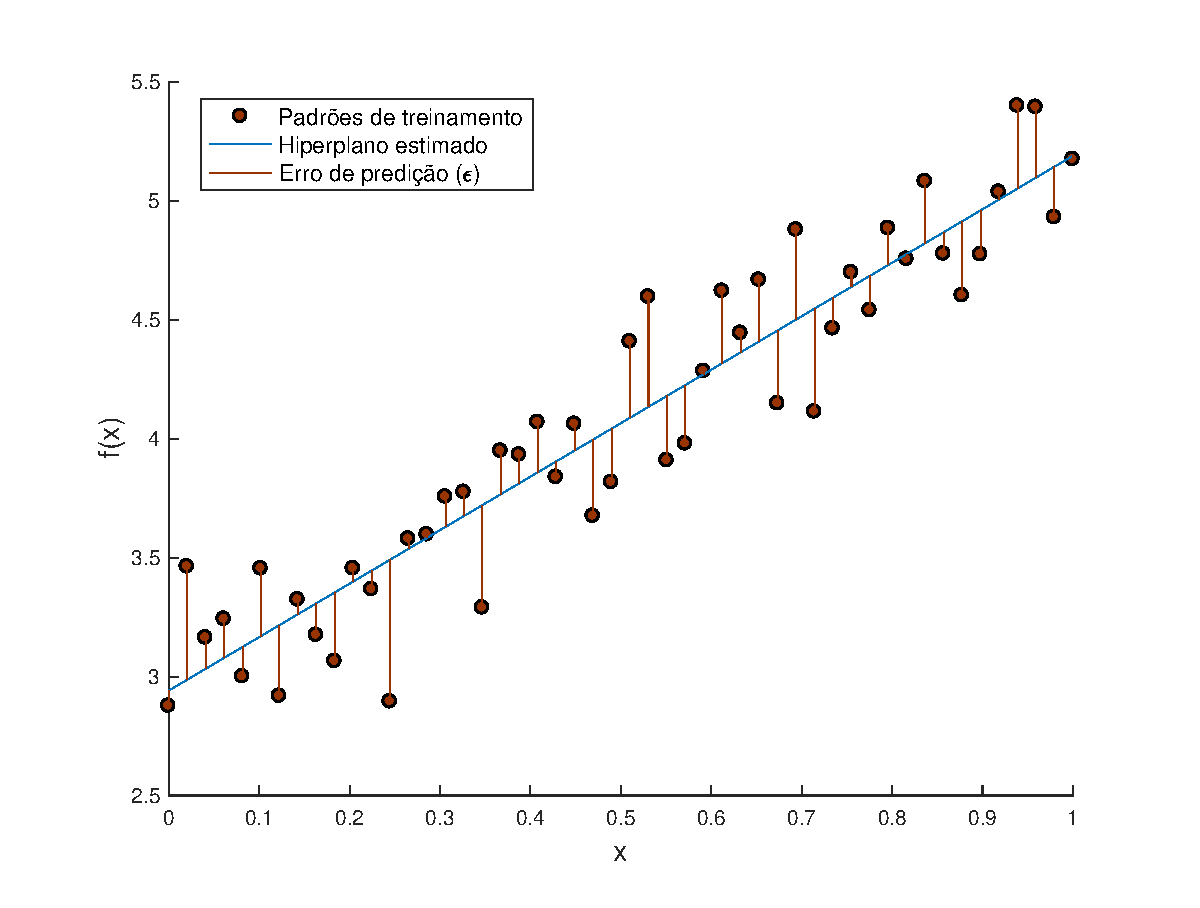
\includegraphics[width=\linewidth]{chapter2/tcc_2D.eps}
        \caption{}
        \label{fig:ch2-linreg1}
    \end{subfigure}%%
    \begin{subfigure}[b]{0.49\linewidth}
        \centering
        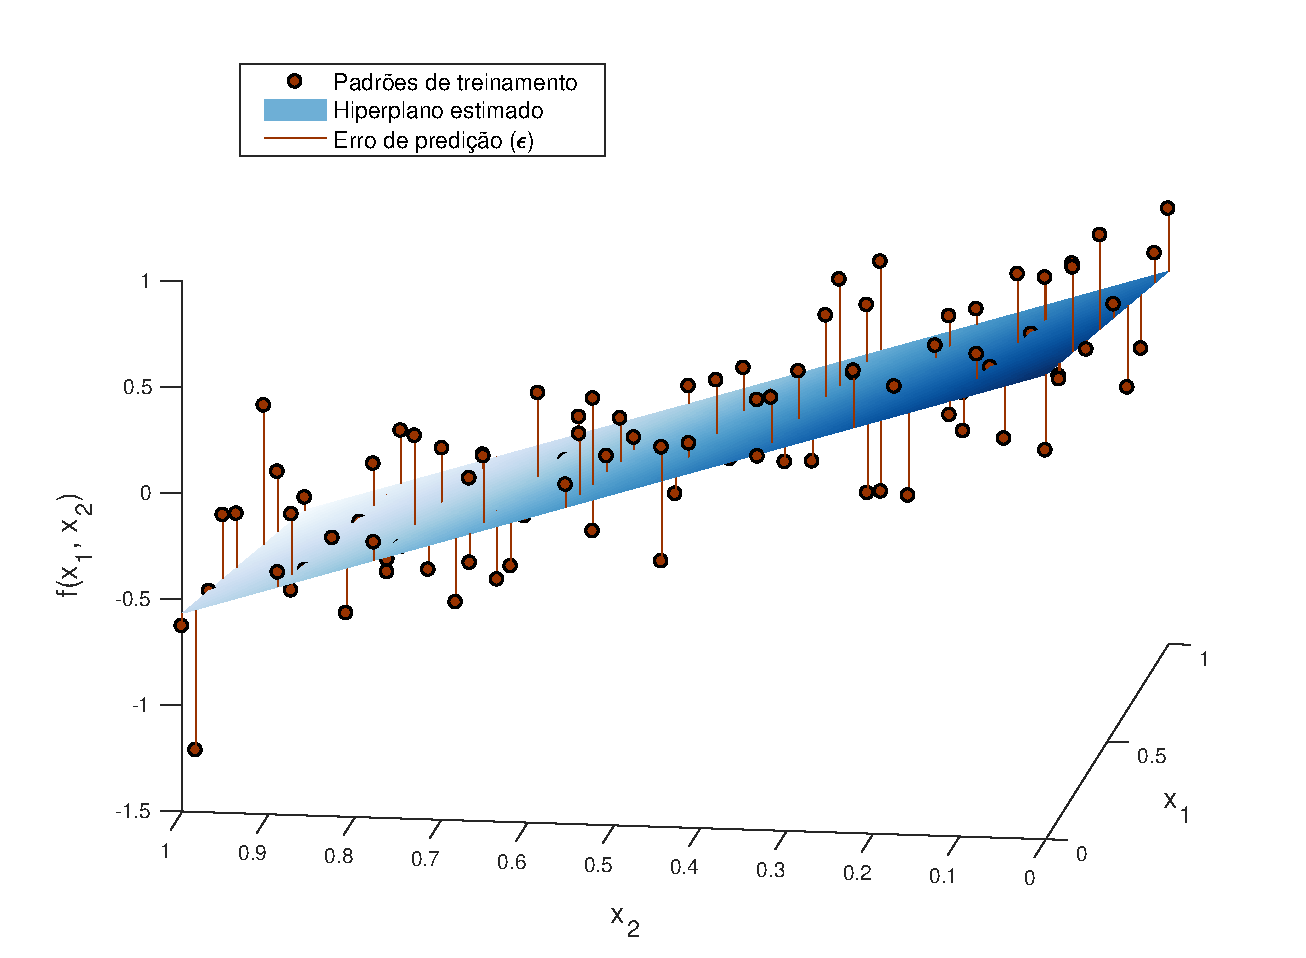
\includegraphics[width=\linewidth]{chapter2/tcc_3D.eps}
        \caption{}
        \label{fig:ch2-linreg2}
    \end{subfigure}
    \centering \makebox[\width]{Fonte: Autor.}
\end{figure}

Embora modelos de regressão sejam capazes de encontrar um hiperplano que represente -- da melhor forma possível -- o comportamento de um objeto de interesse, é comum que não o faça de forma exata. Uma justificativa para esta possibilidade é que modelos de regressão são modelos empíricos; ou seja, são capazes apenas de estimar o comportamento de modelos do mundo real \cite{montgomery2012}. Portanto, é necessário adicionar à equação (\ref{ch2:eq1}) uma medida de erro, que represente a diferença entre os valores observados de $y$ e os valores estimados pelo hiperplano $\mathbf{w}^{\top}\mathbf{x}$. Sumarizando, a equação (\ref{ch2:eq1}) é reescrita como

\begin{equation}
    \label{ch2:eq2}
    y = f(\mathbf{x}) = \mathbf{w}^{\top}\mathbf{x} + \epsilon = \sum_{j=1}^{p}{w_j \cdot x_j} + \epsilon.
\end{equation}

Para encontrar o hiperplano que melhor se ajustará aos padrões de treinamento, é necessário estimar os melhores valores para os parâmetros $w_i$, chamados de \textbf{coeficientes de regressão}. Quando os dados de treinamento são gerados na forma $(\mathbf{x}, f(\mathbf{x}))$, e há $n = p$ padrões linearmente independentes, é possível encontrar os coeficientes de regressão através da solução do sistema linear

\begin{equation}
    \label{ch2:eq3}
    \mathbf{X}\mathbf{w} = \mathbf{y},
\end{equation}

\noindent onde $\mathbf{X}$ é a matriz em que as linhas são formadas pelos padrões de treinamento $\mathbf{x}^{\top}_1,\ldots,\mathbf{x}^{\top}_n$, e $\mathbf{y}$ denota o vetor $[y_1,\ldots,y_n]^{\top}$ \cite{shawe2004}.

Entretanto, podem ocorrer casos em que o número de padrões não é igual a dimensão dos mesmos. Do mesmo modo, pode haver ruído durante o processo de coleta dos padrões, o que torna necessário o uso de outro método para encontrar os coeficientes de regressão. Dos diversos métodos propostos na literatura que são capazes de estimar os valores de cada coeficiente $w_i$, o mais utilizado é o dos mínimos quadrados (do inglês, \textit{least squares}), onde os valores escolhidos para cada coeficiente são aqueles que minimizam a soma de erros quadráticos, $\mathcal{L}(\mathcal{D}, \mathbf{w})$:

\begin{equation}
    \label{ch2:eq4}
    \mathcal{L}(\mathcal{D}, \mathbf{w}) = \sum_{i=1}^{n}{(y_i - f(\mathbf{x}_i))^2} = \sum_{i=1}^{n}{(y_i - \mathbf{w}^{\top}\mathbf{x}_i)^2} = \sum_{i=1}^{n}{\epsilon_{i}^2},
\end{equation}

\noindent onde $\epsilon_{i}^2$ denota o erro quadrático, ou perda quadrática, da estimativa de $f$ para o padrão $\mathbf{x}_i$. Logo, o aprendizado do modelo resume-se a encontrar o vetor $\mathbf{w}$ que minimiza a perda conjunta sobre os padrões de treinamento.

Utilizando notação matricial, podemos escrever o vetor de erros como

\begin{equation}
    \label{ch2:eq5}
    \boldsymbol{\epsilon} = \mathbf{y} - \mathbf{X}\mathbf{w},
\end{equation}

\noindent o que possibilita reescrever a equação (\ref{ch2:eq4}) como

\begin{align}
    \label{ch2:eq6}
    \mathcal{L}(\mathcal{D}, \mathbf{w})
    &= \boldsymbol{\epsilon}^{\top}\boldsymbol{\epsilon} \notag \\
    &= (\mathbf{y} - \mathbf{X}\mathbf{w})^{\top}(\mathbf{y} - \mathbf{X}\mathbf{w}) \notag \\
    &= \mathbf{y}^{\top}\mathbf{y} - \mathbf{w}^{\top}\mathbf{X}^{\top}\mathbf{y} - \mathbf{y}^{\top}\mathbf{X}\mathbf{w} + \mathbf{w}^{\top}\mathbf{X}^{\top}\mathbf{X}\mathbf{w} \notag \\
    &= \mathbf{y}^{\top}\mathbf{y} - 2\mathbf{w}^{\top}\mathbf{X}^{\top}\mathbf{y} + \mathbf{w}^{\top}\mathbf{X}^{\top}\mathbf{X}\mathbf{w}
\end{align}

Minimizar a soma de erros quadrados resume-se a derivar (\ref{ch2:eq6}) em relação a $\mathbf{w}$. Ou seja, o vetor $\mathbf{\hat{w}}$ estimado pelo método dos mínimos quadrados deve satisfazer

\begin{equation}
    \label{ch2:eq7}
    \frac{\partial \mathcal{L}}{\partial\mathbf{w}} = - 2\mathbf{X}^{\top}\mathbf{y} + 2\mathbf{X}^{\top}\mathbf{X}\mathbf{w} = \mathbf{0},
\end{equation}

\noindent que pode ser simplificado como

\begin{equation}
    \label{ch2:eq8}
    \mathbf{X}^{\top}\mathbf{X}\mathbf{w} = \mathbf{X}^{\top}\mathbf{y}.
\end{equation}

As equações (\ref{ch2:eq8}) são conhecidas como equações normais, umas vez que o vetor de erros $\boldsymbol{\epsilon}$ é ortogonal (ou normal) em relação ao hiperplano gerado \cite{bates1988}. Para solucionar as equações normais, podemos multiplicar ambos os lados de (\ref{ch2:eq8}) pela inversa de $\mathbf{X}^{\top}\mathbf{X}$, supondo que a matriz $(\mathbf{X}^{\top}\mathbf{X})^{-1}$ exista. Portanto, o vetor $\mathbf{\hat{w}}$ obtido é

\begin{equation}
    \label{ch2:eq9}
    \mathbf{\hat{w}} = (\mathbf{X}^{\top}\mathbf{X})^{-1}\mathbf{X}^{\top}\mathbf{y}.
\end{equation}

Por fim, a função de predição para novos padrões é dada por

\begin{equation}
    \label{ch2:eq10}
    f(\mathbf{x}) = \mathbf{\hat{w}}^{\top}\mathbf{x}.
\end{equation}

Modelos de regressão linear são bastante utilizados pela simplicidade em sua formulação, que permite fácil modelagem de relacionamentos das variáveis de interesse. Entretanto, existem problemas que possuem quantidades insuficientes de padrões para treinamento, ruído no processo de coleta dos dados, multicolinearidade, entre outros. Essas são algumas dificuldades tipicamente encontradas em problemas mal-condicionados. Uma abordagem frequentemente utilizada é restringir a escolha de funções para aquelas que possuem normas pequenas \cite{shawe2004}. Essa abordagem cria um critério de otimização conhecido como \textit{ridge regression}, discutido na seção \ref{sec:ridge}.

\section{\textit{Ridge regression}} \label{sec:ridge}
O método dos mínimos quadrados possui grande popularidade em áreas como estatística, otimização e aprendizado de máquinas; em grande parte, isso deve-se a simplicidade de sua formulação matemática e à suas propriedades analíticas. Uma das propriedades mais interessantes é obtida através do teorema de Gauss-Markov, o qual diz que os coeficientes estimados pelos mínimos quadrados são os melhores estimadores lineares não-enviesados. Por ``melhores'', diz-se que possuem menor variância entre a classe de estimadores lineares não-enviesados, embora não haja garantia de que essa variância seja pequena \cite{montgomery2012}.

Diversos métodos foram propostos para solucionar este problema e, de modo geral, são chamados de métodos de redução (do inglês, \textit{shrinkage methods}). Um dos mais utilizados é a regressão \textit{ridge} (do inglês, \textit{ridge regression}) originalmente proposta por \apudonline[p. 305]{hoerl1970a}{montgomery2012} e que funciona como um método de penalização da soma de erros quadráticos, correspondendo a solucionar o problema de minimização

\begin{equation}
    \label{ch2:eq11}
    \min_{\mathbf{w}} \mathcal{L}_{\lambda}(\mathcal{D}, \mathbf{w}) = \min_{\mathbf{w}} \lambda \|\mathbf{w}\|^2 + \sum_{i=1}^{n}{(y_i - f(\mathbf{x}_i))^2},
\end{equation}

\noindent onde $\lambda$ é um número positivo que define o balanceamento entre a norma e o erro. Em outras palavras, $\lambda$ opera como um fator de regularização no método dos mínimos quadrados. Esta formulação da \textit{ridge regression} é chamada de formulação primal (ou método primal), pois define o espaço de soluções viáveis com base nas variáveis do problema original.

Seguindo \citeonline{shawe2004}, ao tomar a derivada de (\ref{ch2:eq11}) em relação a $\mathbf{w}$, obtemos as equações

\begin{equation}
    \label{ch2:eq12}
    \mathbf{X}^{\top}\mathbf{X}\mathbf{w} + \lambda\mathbf{w} = (\mathbf{X}^{\top}\mathbf{X} + \lambda\mathbf{I}_n)\mathbf{w} = \mathbf{X}^{\top}\mathbf{y},
\end{equation}

\noindent onde $\mathbf{I}_n$ é a matriz identidade $n \times n$. Neste caso, a matriz $(\mathbf{X}^{\top}\mathbf{X} + \lambda\mathbf{I}_n)$ é sempre invertível, dado que $\lambda > 0$. Dessa forma, o vetor de coeficientes $\mathbf{\hat{w}}$ é

\begin{equation}
    \label{ch2:eq13}
    \mathbf{\hat{w}} = (\mathbf{X}^{\top}\mathbf{X} + \lambda\mathbf{I}_n)^{-1}\mathbf{X}^{\top}\mathbf{y}.
\end{equation}

Solucionar a equação (\ref{ch2:eq13}) para $\mathbf{\hat{w}}$ envolve solucionar um sistema linear de $p \times p$ equações. A complexidade deste método é da ordem $\mathcal{O}(p^3)$, enquanto a função de predição para novos padrões é dada por

\begin{equation}
    \label{ch2:eq14}
    f(\mathbf{x}) = \mathbf{\hat{w}}^{\top}\mathbf{x}.
\end{equation}

\subsection{Formulação dual} \label{subsec:ridge-dual}
A formulação primal da \textit{ridge regression} nos permite inferir que o custo de encontrar os coeficientes $w_i$ depende diretamente da dimensionalidade, $p$, dos padrões. Em casos onde $p$ é muito grande, a solução da equação (\ref{ch2:eq13}) torna-se muito custosa computacionalmente. Entretanto, pode-se desenvolver uma formulação dual através dos multiplicadores de Lagrange, que expressa o vetor $\mathbf{w}$ como uma combinação linear dos padrões de treinamento.

Esta derivação segue os passos descritos por \citeonline{saunders1998}. Primeiramente, devemos reescrever a equação (\ref{ch2:eq11}) como

\begin{equation}
    \label{ch2:eq15}
    \begin{aligned}
        & \text{minimize}
        & & \lambda \|\mathbf{w}\|^2 + \sum_{i=1}^{n}{(y_i - f(\mathbf{x}_i))^2} \\
        & \text{sujeito a}
        & & \{y_i = \mathbf{w}^{\top}\mathbf{x}_i + \epsilon_i\}_{i=1}^{n}.
    \end{aligned}
\end{equation}

Utilizando as restrições descritas em (\ref{ch2:eq15}), podemos escrever o problema em sua forma dual através da construção do lagrangiano, que é dada por

\begin{equation}
    \label{ch2:eq16}
    L(\mathcal{D}, \mathbf{w}, \boldsymbol{\epsilon}, \boldsymbol{\alpha}) = \lambda \|\mathbf{w}\|^2 + \sum_{i=1}^{n}{\epsilon_i^{2} + \sum_{i=1}^{n} \alpha_i(y_i - \mathbf{w}^{\top}\mathbf{x}_i - \epsilon_i)},
\end{equation}

\noindent onde $\epsilon_i = y_i - f(\mathbf{x}_i)$ e $\boldsymbol{\alpha}$ é o vetor de coeficientes de Lagrange. O passo seguinte para obter a solução da equação (\ref{ch2:eq16}) é tomar os gradientes das variáveis primais iguais a zero, seguindo as condições de otimalidade de Karush-Kuhn-Tucker (KKT) \cite{boyd2004}.

Diferenciando $L(\mathcal{D}, \mathbf{w}, \boldsymbol{\epsilon}, \boldsymbol{\alpha})$ em relação a $\mathbf{w}$, obtemos

\begin{equation}
    \label{ch2:eq17}
    \mathbf{w} = \frac{1}{2\lambda} \sum_{i=1}^{n} \alpha_i \mathbf{x}_i.
\end{equation}

\noindent Substituindo (\ref{ch2:eq17}) em (\ref{ch2:eq16}), obtemos

\begin{align}
    \label{ch2:eq18}
    L(\mathcal{D}, \mathbf{w}, \boldsymbol{\epsilon}, \boldsymbol{\alpha}) 
    &= \frac{1}{4\lambda} \sum_{i=1}^{n} \sum_{j=1}^{n} \alpha_i \alpha_j (\mathbf{x}_i^{\top} \mathbf{x}_j) + \sum_{i=1}^{n} \epsilon_i^2 \notag \\
    &+ \frac{1}{2\lambda} \bigg{(}\sum_{i=1}^{n} \alpha_i \mathbf{x}_i\bigg{)}\bigg{(}-\sum_{i=1}^{n} \alpha_i \mathbf{x}_i\bigg{)} + \sum_{i=1}^{n} y_i \alpha_i - \sum_{i=1}^{n} \alpha_i \epsilon_i \notag \\
    &= -\frac{1}{4\lambda} \sum_{i=1}^{n} \sum_{j=1}^{n} \alpha_i \alpha_j (\mathbf{x}_i^{\top} \mathbf{x}_j) + \sum_{i=1}^{n} \epsilon_i^2 + \sum_{i=1}^{n} y_i \alpha_i - \sum_{i=1}^{n} \alpha_i \epsilon_i.
\end{align}

\noindent Diferenciando (\ref{ch2:eq18}) em relação a $\epsilon_i$, obtemos

\begin{equation}
    \label{ch2:eq19}
    \epsilon_i = \frac{\alpha_i}{2}, \quad i=1,\ldots,n.
\end{equation}

\noindent Através da equação (\ref{ch2:eq19}) pode-se inferir que a importância da i-ésima restrição é proporcional a seu respectivo erro. Ao substituir (\ref{ch2:eq19}) em (\ref{ch2:eq18}), temos que

\begin{equation}
    \label{ch2:eq20}
    L(\mathcal{D}, \mathbf{w}, \boldsymbol{\epsilon}, \boldsymbol{\alpha}) = -\frac{1}{4\lambda} \sum_{i=1}^{n} \sum_{j=1}^{n} \alpha_i \alpha_j (\mathbf{x}_i^{\top} \mathbf{x}_j) -\frac{1}{4} \sum_{i=1}^{n} \alpha_i^2 + \sum_{i=1}^{n} y_i \alpha_i.
\end{equation}

\noindent Denotando $K$ como a matriz $n \times n$ dos produtos internos \[ K_{ij} = \mathbf{x}_i^{\top}\mathbf{x}_j, \] e diferenciando (\ref{ch2:eq20}) em relação a $\alpha_i$, obtemos que

\begin{equation}
    \label{ch2:eq21}
    -\frac{1}{2\lambda} K\boldsymbol{\alpha} - -\frac{1}{2} \boldsymbol{\alpha} + \mathbf{y} = \mathbf{0},
\end{equation}

\noindent que é equivalente a 

\begin{equation}
    \label{ch2:eq22}
    \boldsymbol{\alpha} = 2\lambda(K + \lambda\mathbf{I}_n)^{-1}\mathbf{y}.
\end{equation}

\noindent Utilizando a equação (\ref{ch2:eq17}), podemos obter que a função de predição para novos padrões é

\begin{align}
    \label{ch2:eq23}
    f(\mathbf{x}) 
    &= \mathbf{w}^{\top}\mathbf{x} \notag \\
    &= \bigg{(} \frac{1}{2\lambda} \sum_{i=1}^{n} \alpha_i \mathbf{x}_i \bigg{)} \mathbf{x} \notag \\
    &= \frac{1}{2\lambda} \boldsymbol{\alpha} \mathbf{k} \notag \\
    &= \mathbf{y}^{\top}(K + \boldsymbol{\alpha}\mathbf{I}_n)^{-1}\mathbf{k},
\end{align}

\noindent onde $\mathbf{k} = [k_1,\ldots,k_n]^{\top}$ é o vetor dos produtos internos: \[ k_i = \mathbf{x}_i^{\top}\mathbf{x}, \quad i = 1,\ldots,n. \]

\section{O truque do \textit{kernel}} \label{sec:kernel-trick}
Até o presente momento, as formulações dos mínimos quadrados e da \textit{ridge regression} tinham como objetivo encontrar relações lineares entre as variáveis de um problema. As funções que permitem modelar problemas de regressão devem, então, ser lineares ou uma aproximação linear razoável \cite{hastie2009}. Contudo, a grande maioria dos problemas do mundo real possui natureza não-linear, de forma que estimativas mais precisas de $y$ só podem ser obtidas através do uso de uma função (ou combinação de funções) não-linear.

Uma estratégia interessante que tornou-se bastante popular, consiste em mapear os padrões para um espaço de Hilbert de alta (ou até infinita) dimensão, onde as relações tornam-se lineares e, consequentemente, seja possível aplicar modelos como a \textit{ridge regression}. Os mapeamentos considerados são da forma

\begin{equation}
    \label{ch2:eq24}
    \mathbf{\phi} : \mathbf{x} \mapsto \mathbf{\phi}(\mathbf{x}) \in \mathcal{H}.
\end{equation}

% \noindent O objetivo do mapeamento $\phi$ é converter o problema não-linear em um problema linear.
\noindent A consequência disso é vista sobre o conjunto de treinamento, que deve ser reformulado como $\mathcal{D} = \{(\phi(\mathbf{x}_i), y_i)\}^{n}_{i=1}$. Dessa forma, o modelo descrito na equação (\ref{ch2:eq2}) torna-se

\begin{equation}
    \label{ch2:eq25}
    y = f(\mathbf{x}) = \mathbf{w}^{\top} \phi(\mathbf{x}) + \epsilon = \sum_{j=1}^{p}{w_j \cdot \phi(x_j)} + \epsilon
\end{equation}

O uso da ``versão primal'' da \textit{ridge regression}, apesar de possível, pode tornar-se inviável em termos computacionais, por causa da ``maldição da dimensionalidade'' (do inglês, \textit{curse of dimensionality}). Em suma, o fato de haver funções não-lineares que operam em espaços de dimensão infinita torna inviável o uso da \textit{ridge regression} em sua forma primal, pois o modelo de computação atual não opera com o conceito de infinitude. Entretanto, a formulação dual traz a grande vantagem de não precisar representar os padrões de forma explícita no espaço $ \mathcal{H}$, chamado de espaço de características; são necessários apenas os produtos internos entre os pares de padrões

\begin{equation}
    \label{ch2:26}
    K_{ij} = \phi(\mathbf{x}_i)^{\top} \phi(\mathbf{x}_j).
\end{equation}

À esse atalho é dado o nome truque do \textit{kernel} (do inglês, \textit{kernel trick}). A Figura \ref{fig:kernel-trick} ilustra a ideia básica do truque do \textit{kernel}, onde os padrões $\mathbf{x} \in \mathcal{X}$ são mapeados para um espaço de Hilbert, $\mathcal{H}$, onde relações lineares são descobertas e consequentemente, equivalem a predições precisas no espaço original, $\mathcal{X}$. Uma função que realiza o mapeamento dos padrões para um espaço de Hilbert é chamada \textbf{função de \textit{kernel}}.

\begin{definition}[Função de \textit{Kernel}]
\label{def:kernel-function}
Um \textit{kernel} é uma função $\kappa$ que para todo $\mathbf{x}, \mathbf{z} \in \mathcal{X}$ satisfaz \[\kappa(\mathbf{x}, \mathbf{z}) = \phi(\mathbf{x})^{\top} \phi(\mathbf{z}), \] onde $\phi$ é uma função de mapeamento de $\mathcal{X}$ para um espaço característico $\mathcal{H}$ \[\mathbf{\phi} : \mathbf{x} \mapsto \mathbf{\phi}(\mathbf{x}) \in \mathcal{H}.\]
\end{definition}

\begin{figure}[H]
    \centering
    \caption{Ilustração da ideia básica em métodos de \textit{kernel}. Ao escolher um mapeamento adequado, os padrões são embutidos em um RKHS, $\mathcal{H}$, onde as relações são lineares. Predições no espaço $\mathcal{H}$ equivalem, então, a predições no espaço original, $\mathcal{X}$. A função de mapeamento, $\phi$, pode ser definida implicitamente através da escolha do \textit{kernel}.}
    \label{fig:kernel-trick}
    \includegraphics[width=\linewidth]{figures/images/kernel-example.png}
    \makebox[\width]{Fonte: Autor.}
\end{figure}

Utilizando-se do truque do \textit{kernel}, podemos redefinir a equação (\ref{ch2:eq16}), referente ao lagrangiano da \textit{ridge regression}, para

\begin{equation}
    \label{ch2:27}
    L(\mathcal{D}, \mathbf{w}, \boldsymbol{\epsilon}, \boldsymbol{\alpha}) = \lambda \|\mathbf{w}\|^2 + \sum_{i=1}^{n}{\epsilon_i^{2} + \sum_{i=1}^{n} \alpha_i(y_i - \mathbf{w}^{\top}\phi(\mathbf{x}_i) - \epsilon_i)}
\end{equation}

Finalmente, a nova função de predição é descrita como

\begin{equation}
    \label{ch2:eq29}
    f(\mathbf{x}) = \mathbf{y}^{\top}(K + \boldsymbol{\alpha}\mathbf{I}_n)^{-1}\mathbf{k},
\end{equation}

\noindent onde $K$ é a matriz de produtos internos dos vetores $\phi(\mathbf{x}_i), \ldots, \phi(\mathbf{x}_n)$, resultados da aplicação da função de \textit{kernel} $\kappa$ sobre os padrões de treinamento, e $\mathbf{k}$ é o vetor de produtos internos: \[ k_i = \phi(\mathbf{x}_i)^{\top}\mathbf{x}, \quad\quad i = 1,\ldots,n. \]

Da equação (\ref{ch2:eq29}) surge o modelo conhecido como \textit{kernel ridge regression} (KRR), que será utilizado no decorrer desta monografia.

Vários métodos de \textit{kernel} tornam-se um problema de otimização no espaço de Hilbert, $\mathcal{H}$. Do teorema do representante (\textit{representer theorem}) \cite{aronszajn1950,scholkopf2001} segue que, embora o problema seja definido em um RKHS de alta (ou infinita) dimensão, sua solução permanece no subespaço $p$-dimensional definido pela extensão dos \textit{kernels} centrados nos $n$ padrões de treinamento. Considerando os cômputos de $\phi$ da ordem $\mathcal{O}(n)$, pode-se afirmar que o custo assintótico do cômputo dos coeficientes de Lagrange é da ordem $\mathcal{O}(n^3 + n^2p)$, enquanto o custo de predição é da ordem $\mathcal{O}(np)$. Apesar de possuir um custo assintótico maior, a formulação dual permite computar os produtos internos de modo mais eficiente que a formulação primal, já que não é necessário computar o mapeamento $\phi$ de maneira explícita. Dessa forma, a dual apresenta-se como uma representação mais eficiente que a primal.

% Para uma visão mais aprofundada (e teórica) sobre métodos de \textit{kernel}, recomenda-se a leitura dos textos \cite{smola1998learning,shawe2004,hofmann2008kernel,scholkopf2001}.

% O próprio termo \textit{kernel} pode conter diversos significados, quando aplicado em diferentes contextos.

% \section{Algumas propriedades de \textit{kernels}} \label{sec:kernel-properties}

\section{\textit{Genetic Kernels for Regression} (Proposta)} \label{sec:gkr}
Encontrar uma função de \textit{kernel} que se adapte a um determinado problema é um estágio crítico no desenvolvimento de métodos de aprendizagem baseados em \textit{kernels}. Isso se deve muito ao fato da necessidade de haver conhecimento \textit{a priori} sobre o problema \cite{shawe2004}. De acordo com \citeonline{scholkopf2001}, a própria escolha do \textit{kernel} representa conhecimento sobre o problema e sua solução. Como já mencionado no Capítulo \ref{chapter:introduction}, uma abordagem bastante utilizada na comunidade acadêmica é utilizar \textit{kernels} já consolidados na literatura, apenas realizando uma busca pelo seus melhores conjuntos de parâmetros. A Tabela \ref{tab:commom-kernels} apresenta uma lista das principais funções de \textit{kernels} utilizadas e seus respectivos parâmetros.

\begin{table}[H]
    \caption{Funções de \textit{kernel} mais populares na literatura.}
    \begin{center} \label{tab:commom-kernels}
        \begin{tabular}{l@{\hskip 20pt}l}
            \hline\noalign{\smallskip}
            \textbf{\textit{Kernel}} & \textbf{Descrição} \\
            \noalign{\smallskip}
            \hline
            \noalign{\smallskip}
            Linear		& $\kappa({\mathbf x}$,${\mathbf z}$) $= \mathbf{x}^{\top}\mathbf{z}$ \\
            RBF	        & $\kappa({\mathbf x}$,${\mathbf z}$) $= e^{-\|\mathbf{x} - \mathbf{z}\|^2 / \sigma^2}$, onde $\sigma$ é uma constante. \\
            Polinomial	& $\kappa({\mathbf x}$,${\mathbf z}$) $= (\mathbf{x}^{\top}\mathbf{z} + 1)^d$, onde $d$ é o grau do polinômio. \\
            \hline
        \end{tabular}
    \end{center}
    \begin{center}
        \makebox[\width]{Fonte: \citeonline{ajalmar2011}}.
    \end{center}
\end{table}

% Como alternativa, duas outras abordagens são encontradas na literatura. A primeira concentra-se no aprendizado de \textit{kernels} a partir do conjunto de dados. Essa abordagem funciona através da definição de um conjunto de \textit{kernels}
% (\textit{Multiple Kernel Learning}, MKL)

Criar \textit{kernels} que adaptem-se a problemas específicos é uma opção mais conveniente, pois o(a) projetista de um modelo baseado em \textit{kernels} não necessita verificar qual \textit{kernel} é melhor para o problema que deve ser solucionado. Entretanto, projetar uma função de \textit{kernel} demanda muito conhecimento acerca do problema, de forma que torna-se muito custoso (em termos de tempo dispendido) realizar esta tarefa manualmente. Uma alternativa é a utilização da construção em blocos. Esse modelo de construção utiliza operadores de fechamento sobre as funções de \textit{kernel} que permite que novas funções sejam geradas a partir da combinação de outras já conhecidas. A Proposição \ref{prop:1}, adaptada de \cite{shawe2004} lista três operadores de fechamento que garantem a construção de novas funções de \textit{kernel} válidas.
% Uma alternativa, que vem ganhando bastante popularidade em anos recentes, é a criação de funções de \textit{kernel} específicas para determinados tipos de problemas. Uma forma possível de criação de novos \textit{kernels} é a utilização da construção em blocos. Esse modelo de construção utiliza propriedades de fechamento sobre as funções de \textit{kernel} que permite que novas funções sejam geradas a partir da combinação de outras já conhecidas. A Proposição \ref{prop:1}, adaptada de \cite{shawe2004} lista três operações de fechamento que garantem a construção de novas funções de \textit{kernel} válidas.

\begin{proposition}[Propriedades de fechamento]
    \label{prop:1}
    Sejam $\kappa_1$ e $\kappa_2$ dois kernels sobre $\mathbf{X} \times \mathbf{X}, \mathbf{X} \subseteq
    \mathbb{R}^n$ e $a \in \mathbb{R}^+$. Então as seguintes funções são kernels

    \begin{enumerate}[label=(\roman*)]
        \item $\kappa(\mathbf{x},\mathbf{z}) = \kappa_1(\mathbf{x},\mathbf{z}) + \kappa_2(\mathbf{x},\mathbf{z})$,
        \item $\kappa(\mathbf{x},\mathbf{z}) = \kappa_1(\mathbf{x},\mathbf{z}) \times \kappa_2(\mathbf{x},\mathbf{z})$,
        \item $\kappa(\mathbf{x},\mathbf{z}) = a \cdot \kappa_2(\mathbf{x},\mathbf{z})$.
        % \item $k(\mathbf{x},\mathbf{z}) = e^{\kappa_1(\mathbf{x},\mathbf{z})}$.
    \end{enumerate}
\end{proposition}

A proposta deste trabalho, denominada \textit{Genetic Kernels for Regression} (GKR), baseia-se em PG para encontrar \textit{kernel}(\textit{s}) para quaisquer problemas de regressão a serem solucionados pelo método KRR. Como entrada, o GKR recebe o parâmetro de regularização $\lambda$, e um conjunto de dados de treinamento $\mathcal{D}$. Ao fim de sua realização, o algoritmo retorna o melhor \textit{kernel} encontrado, que será usado na construção do modelo de predição final.

Inicialmente, uma população de soluções é construída de forma aleatória, tal que cada indivíduo representa um \textit{kernel} construído utilizando as propriedades apresentadas na Proposição \ref{prop:1} e os \textit{kernels} apresentados na Tabela \ref{tab:gkr-kernels}. A avaliação dos indivíduos se dá através da raiz da média dos erros quadráticos (\textit{Root Mean Squared Error}, RMSE). As gerações seguintes são criadas a partir da aplicação dos operadores genéticos (seção \ref{sec:genetic-operators}) sobre os melhores indivíduos da atual população, escolhidos com base em seus valores de aptidão. Este processo é repetido até que um dos critérios de parada seja atendido. Ao fim do processo evolutivo, o melhor indivíduo da população final é escolhido para a criação do modelo final. A Figura \ref{fig:gkr-overview} apresenta uma visualização do fluxo de trabalho do GKR.

\begin{figure}[H]
    \caption{Fluxo de trabalho do algoritmo GKR.}
    \centering
    \label{fig:gkr-overview}
    \begin{tikzpicture}[node distance = 4cm, auto,
        decision/.style={diamond, draw, fill=my_gray, text width=3em, text=white, aspect=1, text centered, node distance=3cm, inner sep=0pt},
        block inside/.style={rectangle, draw, fill=none, text width=8em, text centered, rounded corners, minimum height=3em}]

        \node [block] (dataset) {\scriptsize conjunto de dados de treinamento};
        \node [block, right of=dataset] (lambda) {\scriptsize parâmetro de regularização};
        \node [block inside, node distance=2.5cm, below of=dataset] (init) {\scriptsize criar população inicial de soluções};
        \node [block inside, node distance=2.5cm, below of=init] (fitness) {\scriptsize avaliar população de indivíduos};
        \node [decision, below of=fitness, node distance=2.5cm] (decide) {\scriptsize \textbf{D}};
        \node [block inside, right of=decide, node distance=5cm] (selection) {\scriptsize selecionar indivíduos};
        \node [block inside, above of=selection, node distance=2.5cm] (update) {\scriptsize atualizar população};
        \node [block inside, right of=update, node distance=4.5cm] (breeding) {\scriptsize aplicar operadores genéticos};
        \node [block inside, below of=decide, node distance=2.5cm] (bestsofar) {\scriptsize melhor indivíduo};
        \node [block, below of=bestsofar, node distance=2.5cm] (kernel) {\scriptsize função de \textit{kernel}};
        \node [decision, right of=bestsofar, text width=2em, node distance=9.2cm] (decide2) {\tiny \textbf{D}};
        \node [draw=none, right of=decide2, node distance=1.3cm, text width=4em, text centered] (end) {\tiny terminar busca?};

        \draw[very thick, dashed, rounded corners] ($(init.north west)+(-0.4,0.4)$) rectangle ($(end.south east)+(0.2,-0.7)$) node[text=black] at ($(breeding.north east)+(-0.2,3.2)$, 0) {\scriptsize \textbf{GKR}};
        \path [line] (dataset) -- (init);
        \path [line] (lambda) |- (init);
        \path [line] (init) -- (fitness);
        \path [line] (fitness) -- (decide);
        \path [line] (selection.east) -| (breeding.south);
        \path [line] (decide) -- node {\tiny não} (selection);
        \path [line] (decide) -- node {\tiny sim} (bestsofar);
        \path [line] (breeding) -- (update);
        \path [line] (update) -- (fitness);
        \path [line] (bestsofar) -- (kernel);
    \end{tikzpicture}
    \makebox[\width]{Fonte: Autor.}
\end{figure}

% Um potencial problema que pode surgir durante a execução do algortimo da PG, é o que muito autores chamam de \textit{bloat}. Esse fenômeno faz com as árvores geradas cresçam sem que se tenha aumento na peformance. Por essa razão, pretende-se utilizar o método de seleção \textit{lexictour}, que tem preferência por indivíduos de menor tamanho caso haja empate de performance entre vários indivíduos.

% Para determinar o quão apto é um indivíduo, uma validação cruzada será utilizada sobre seu RMSE (\textit{root mean squared error}). Antes do processo de evolução de uma geração iniciar, algumas configurações importantes são feitas. O conjunto de dados é dividido em dois subconjuntos: treinamento e teste. O conjunto de treinamento, então, é dividido em 10 partes (\textit{folds}). O treinamento de cada indivíduo é executado durante 10 iterações, sempre deixando um \textit{fold} como um conjunto de validação independente. A aptidão de um indivíduo é dada pela média das 10 validações.

% Nosso método terá sua performance comparada com uma SVM treinada com kernels clássicos (linear, gaussiano e polinomial) e as redes neurais MLP e RBF. Vale salientar que o processo de validação cruzada é o mesmo para todas as técnicas, ou seja, todas são treinadas, validadas e testadas com a mesma divisão do conjunto de dados. Essa escolha permite que as comparações de performance sejam mais precisas.

\subsection{Representação genética e população inicial}
Como já discutido no Capítulo \ref{chapter:genetic-programming}, a representação genética de um indivíduo é uma das partes cruciais no projeto de um algoritmo de PG. Anteriormente à decisão de qual estrutura será escolhida para representação de um indivíduo, é necessário que se decida qual será o conjunto primitivo a ser utilizado; ou seja, é necessário a definição dos conjuntos de funções e terminais. O conjunto de terminais é composto pelo conjunto de dados específico de cada problema, representado pela matriz $\mathbf{X}$, das variáveis de cada \textit{kernel} (tais como $\sigma$, a abertura da gaussiana), e de constantes efêmeras. O conjunto de funções escolhido é uma união entre os operadores apresentados na Proposição \ref{prop:1} e os \textit{kernels} listados na Tabela \ref{tab:gkr-kernels}.

\begin{table}[H]
    \caption{Funções de \textit{kernel} utilizados pelo GKR.}
    \begin{center} \label{tab:gkr-kernels}
        {
        \def\arraystretch{1.8}\tabcolsep=10pt
        \begin{tabular}{l@{\hskip 18pt}l}
            \hline\noalign{\smallskip}
            \textbf{\textit{Kernel}} & \textbf{Equação} \\
            \noalign{\smallskip}
            \hline
            \noalign{\smallskip}
            Cauchy 		            & $\kappa(\mathbf{x},\mathbf{z}) = \frac{1}{1 + \frac{\|\mathbf{x} - \mathbf{z}\|^2}{\sigma^2}}$ \\
            Exponential             & $\kappa(\mathbf{x},\mathbf{z}) = e^{-\frac{\|\mathbf{x} - \mathbf{z}\|}{\sigma^2}}$ \\
            Inverse Multiquadratic  & $\kappa(\mathbf{x},\mathbf{z}) = \frac{1}{\sqrt{\|\mathbf{x} - \mathbf{z}\|^2 + c^2}}$ \\
            Laplace		            & $\kappa(\mathbf{x},\mathbf{z}) = e^{-\frac{\|\mathbf{x} - \mathbf{z}\|}{\sigma}}$ \\
            Linear		            & $\kappa(\mathbf{x},\mathbf{z}) = \mathbf{x}^{\top}\mathbf{z}$ \\
            Multiquadratic          & $\kappa(\mathbf{x},\mathbf{z}) = \sqrt{\|\mathbf{x} - \mathbf{z}\|^2 + c^2}$ \\
            Polynomial	            & $\kappa(\mathbf{x},\mathbf{z}) = (\mathbf{x}^{\top}\mathbf{z} + 1)^d$ \\
            Rational Multiquadratic & $\kappa(\mathbf{x},\mathbf{z}) = 1 - \frac{\|\mathbf{x} - \mathbf{z}\|^2}{\|\mathbf{x} - \mathbf{z}\|^2 + c^2}$ \\
            RBF	                    & $\kappa(\mathbf{x},\mathbf{z}) = e^{-\frac{\|\mathbf{x} - \mathbf{z}\|^2}{\sigma^2}}$ \\
            Sigmoid         		& $\kappa(\mathbf{x},\mathbf{z}) = \tanh(a\mathbf{x}^{\top}\mathbf{z} + 1)$ \\
            \hline
        \end{tabular}
    }
    \end{center}
    \begin{center}
        \makebox[\width]{Fonte: Autor.}
    \end{center}
\end{table}

Vale salientar que, uma vez que as funções de \textit{kernel} recebem dois vetores como entrada (além de seu conjunto de parâmetros), é natural que se utilize uma matriz extra, $\mathbf{Z}$, que represente os padrões $\mathbf{z}$. Entretanto, como essas funções computam valores de similaridade entre padrões de um mesmo conjunto, tem-se que $\mathbf{Z} = \mathbf{X}$. A escolha pela utilização de duas matrizes, ao invés de apenas uma, é puramente por harmonia com a definição de função de \textit{kernel}. Assim, é possível a utilização apenas da matriz $\mathbf{X}$.

A representação genética de um indivíduo é a padrão da PG: árvores sintáticas. Para fins de exemplificação, a Figura \ref{fig:kernel-tree} mostra uma árvore que representa o kernel $Polynomial(\mathbf{X}, \mathbf{Z}, 7) + Linear(\mathbf{X}, \mathbf{Z})$.

Para criação da população inicial, foi utilizada a abordagem STGP. A justificativa para essa escolha encontra-se no fato de que, dado a natureza estocástica da PG, árvores sintaticamente inválidas podem ser criadas. Portanto, a STGP fornece um arcabouço robusto para definição de restrições dos tipos que um nó pode ter. Observe a Figura \ref{fig:kernel-tree} como exemplo: enquanto o nó que contém o \textit{kernel} linear só pode receber como entrada duas matrizes que representam o conjunto de dados, o kernel \textit{polinomial} pode receber uma entrada extra (o grau do polinômio, que possui valor inteiro). A Tabela \ref{tab:stgp-constraints} lista as restrições utilizadas para que o GKR crie árvores sintaticamente válidas.

% Tanto o processo de criação de uma árvore quanto o de alteração através dos operadores genéticos, deve obedecer a essas restrições, mantendo a árvore consistente.

% A população inicial é criada utilizando uma combinação das propriedades de fechamendo e das restrições de STGP para criar novas funções kernel válidas e que permaneçam consistentes ao longo do processo de evolução. A consistência de cada indivíduo é mantida porque em STGP, além das restrições padrões da PG, novas restrições são adicionadas a cada nó.

\begin{figure}[H]
    \caption{Exemplo de \textit{kernel} que pode ser criado pelo GKR. A árvore sintática representa a função $Pol(\mathbf{X}, \mathbf{Z}, 7) + Lin(\mathbf{X}, \mathbf{Z})$, onde $Pol=Polynomial$ e $Lin=Linear$.}
    \label{fig:kernel-tree}
    \begin{center}
        \begin{tikzpicture}[->,>=stealth',auto,
            black/.style={fill=my_black},
            red/.style={fill=my_red},
            default/.style={draw, circle, text=white},
            level 1/.style={sibling distance=50mm},
            level 2/.style={sibling distance=20mm}]
            \node [arn_r, default, black] {+}
            child{ node [arn_r, default, black] {Pol} 
                child{ node [arn_r, default, red] {$\mathbf{X}$} }
                child{ node [arn_r, default, red] {$\mathbf{Z}$} }
                child{ node [arn_r, default, red] {$\mathbf{7}$} }
            }
            child{ node [arn_r, default, black] {Lin}
                child{ node [arn_r, default, red] {$\mathbf{X}$} }
                child{ node [arn_r, default, red] {$\mathbf{Z}$} }
            };
        \end{tikzpicture}
    \end{center}
    \begin{center}
        \makebox[\width]{Fonte: Autor.}
    \end{center}
\end{figure}

\begin{table}[H]
    \caption{Restrições utilizadas pelo GKR para garantir que as árvores criadas sejam sintaticamente válidas.}
    \begin{center} \label{tab:stgp-constraints}
        \begin{tabular}{C@{\hskip 15pt}l}
            \hline\noalign{\smallskip}
            \textbf{Nó} & \textbf{Tipo} \\
            \noalign{\smallskip}
            \hline
            \noalign{\smallskip}
            $\sigma$ & Ponto flutuante \\
            $\mathbf{X}$ e $\mathbf{Z}$ & Matriz de pontos flutuantes \\
            $a$, $c$ e $d$ & Número inteiro \\
            \textit{Kernels} da Tabela \ref{tab:gkr-kernels} & \textit{kernel-function} \\
            Operadores da Proposição \ref{prop:1} & \textit{kernel-operator} \\
            \hline
        \end{tabular}
    \end{center}
    \begin{center}
        \makebox[\width]{Fonte: Autor.}
    \end{center}
\end{table}

\subsection{Função de aptidão e método de seleção}
Para o cálculo da aptidão de um indivíduo, é necessário que sejam computadas predições sobre um conjunto de dados não utilizado durante o treinamento. Isso é realizado através da separação do conjunto de dados de treinamento em dois subconjuntos: treinamento e validação. Detalhes sobre a metodologia de separação podem ser encontrados no Capítulo \ref{chapter:simulations}. A função de aptidão escolhida é a \textit{root mean square error} (RMSE):

\begin{equation}
    \label{ch3:eq29}
    RMSE = \sqrt{\frac{1}{n}\sum_{i=1}^{n}{(y_i - f(\mathbf{x}_i))^2}}
\end{equation}

Naturalmente, poderia ser utilizada a aptidão padronizada (veja seção \ref{sec:fitness-functions}). Entretanto, foi escolhido a aptidão ajustada por dois motivos: (\textit{i}) permite uma melhor separação entre as boas soluções das ótimas soluções, levando a um direcionamento mais preciso na busca pelo melhor indivíduo; e (\textit{ii}) permite usar o algoritmo padrão de PG, onde os melhores indivíduos são aqueles que possuem maiores valores de aptidão.

O método de seleção utilizado foi a seleção por torneio lexicográfico, proposto por \citeonline{luke2002}. Este operador modifica a seleção por torneio tradicional ao preferir árvores de menor profundidade quando dois ou mais indivíduos possuem o mesmo valor de aptidão (ou mesmo \textit{rank}). Este é um operador de seleção que vem sendo bastante utilizado no combate ao crescimento desenfreado do tamanho de um indivíduo, conhecido como \textit{bloat growth} (veja seção \ref{sec:bloat-growth}).

\subsection{Operadores genéticos}
Os operadores genéticos escolhidos são os mesmos descritos na seção \ref{sec:genetic-operators}.

\subsection{Critério de parada}
O algoritmo sempre é encerrado quando ocorre, pelo menos, uma das duas situações a seguir: (\textit{i}) um número predeterminado de gerações é atingido ou (\textit{ii}) a função de aptidão atinge seu valor máximo (ou seja, foi encontrado o \textit{kernel} ideal).
